\chapter{Introdução}
% \addcontentsline{toc}{chapter}{1\hspace{1em}Introdução}
% \setcounter{chapter}{1}

\section{Conceitos básicos}
Esta seção apresenta alguns dos termos comumente utilizados na gestão de receitas no transporte ferroviário de passageiros, além de aprofundar-se em conceitos específicos que frequentemente geram confusão entre si.

\begin{description}[style=unboxed, leftmargin=0cm]

	\item[Viagem:] Um trem programado para uma data específica é denominado "viagem". Uma viagem inclui uma estação de partida (estação de origem) e uma estação de chegada (estação de destino final). Exemplo: O trem \#03450-1 de 12 de janeiro de 2024 é uma viagem:

	      \begin{figure}[H]
		      \begin{center}
			      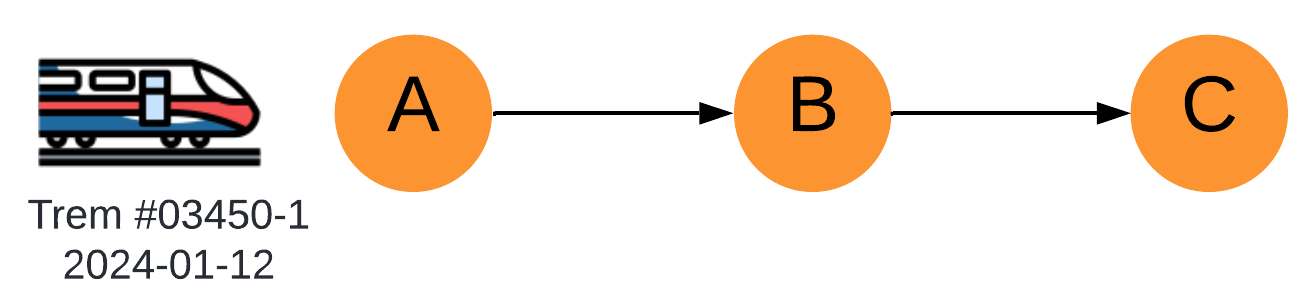
\includegraphics[scale=0.12]{img/viagem.png}
			      \caption{Representação de viagem}
			      \label{fig: viagem}
		      \end{center}
	      \end{figure}
	      \vspace{-1cm}

	\item[Trecho:] Um trecho é uma conexão direta entre duas estações,também pode ser denominado como origem-destino. Além, será dito que um trecho é adjacente se, e somente se, não houver estações intermediárias entre elas; caso contrário, serão não adjacentes. Por exemplo, o trecho AC é ñao adjcente e os trechos AB e BC são adjacentes. É importante aclarar que que os trechos não adjacentes podem conter outros trechos, tanto adjacentes quanto não adjacentes.

	      \begin{figure}[H]
		      \begin{center}
			      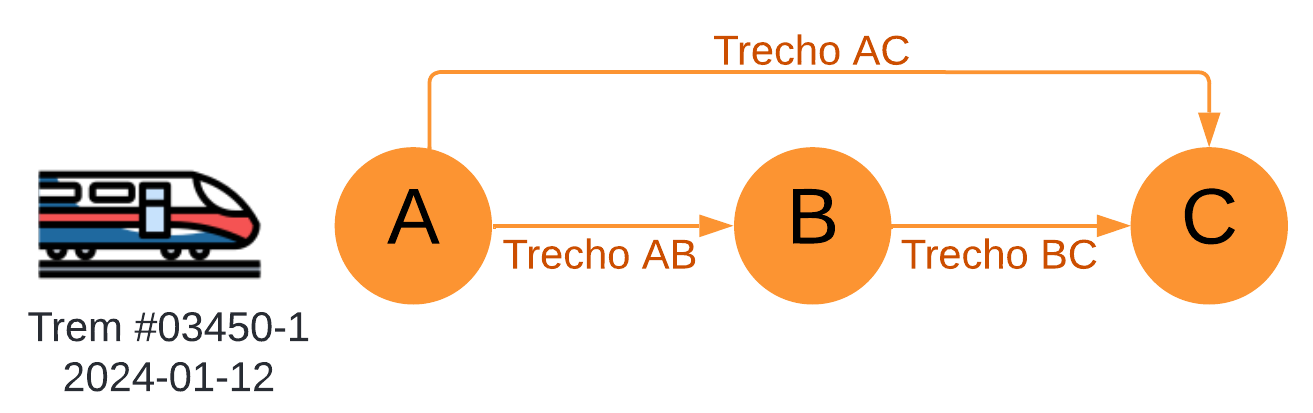
\includegraphics[scale=0.12]{img/trecho.png}
			      \caption{Representação de trechos}
			      \label{fig: trecho}
		      \end{center}
	      \end{figure}
	      \vspace{-1cm}

	\item[Itinerário:] Um itinerário é uma combinação única de origem, destino, horário de partida e trem. Um itinerário pode consistir em um ou mais trechos, e uma viagem pode englobar um ou mais itinerários.

	      \begin{figure}[H]
		      \begin{center}
			      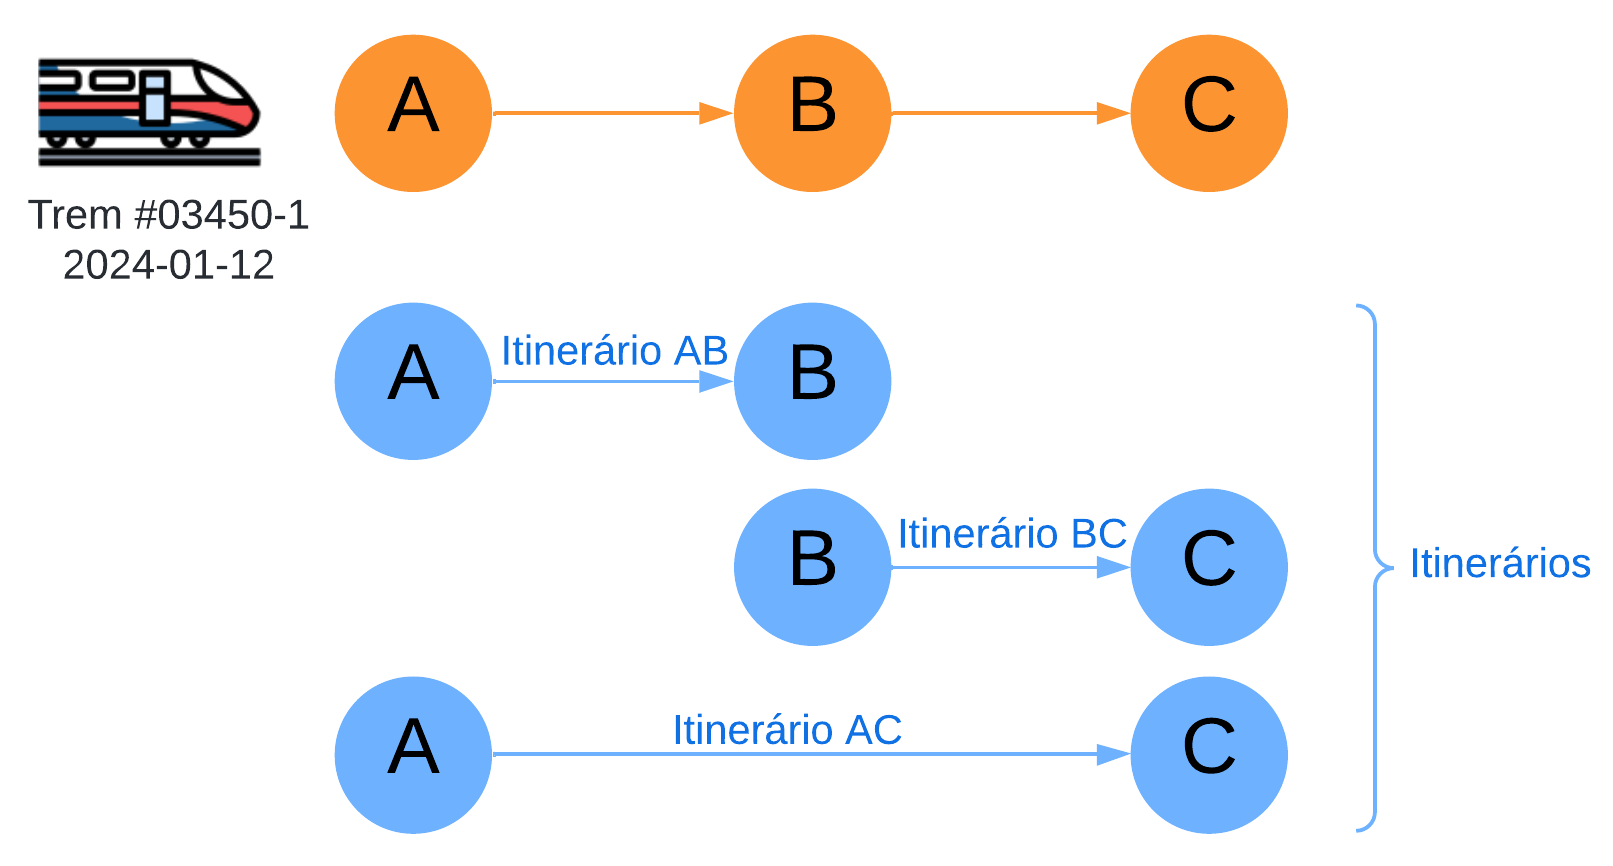
\includegraphics[scale=0.12]{img/itinerario.png}
			      \caption{Representação de itinerários}
			      \label{fig: itinerario}
		      \end{center}
	      \end{figure}
	      \vspace{-1cm}

	\item[Classes de controle:] Uma classe de controle é um produto oferecido por um operador de transporte a passageiros potenciais por um preço específico. As classes de controle também são conhecidas como classes tarifárias, produtos tarifários ou classes de reservas. Uma classe de controle define os benefícios e/ou restrições que o passageiro terá como resultado do preço pago pelo bilhete.

	\item[Horizonte de reserva:] É o período de tempo entre o momento em que os bilhetes para o trem em questão são disponibilizados para venda pela primeira vez e a data de partida do trem. O horizonte de reserva geralmente é discretizado por dias, de forma que cada período representa um dia específico antes da partida (DBD). Frequentemente, realizamos uma agregação temporal para reduzir o tamanho do horizonte de reserva, selecionando alguns DBD específicos como pontos de controle (CP). Nesse contexto, o horizonte de contabilização é discretizado por períodos, onde o tamanho de cada período corresponde ao intervalo de tempo entre dois CP consecutivos.

	      \begin{figure}[H]
		      \begin{center}
			      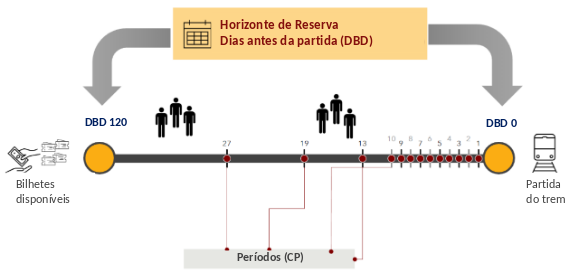
\includegraphics[scale=0.53]{img/h_reserva.png}
			      \caption{Representação do horizonte de reserva}
			      \label{fig: h_reserva}
		      \end{center}
	      \end{figure}
	      \vspace{-1cm}

	\item[Reservas:] As reservas representam o número de assentos protegidos para atender à demanda potencial de uma classe de controle específica em um determinado itinerário, durante um período específico do horizonte de reserva. O tamanho da reserva é definido no processo de otimização, considerando a demanda potencial do itinerário e da classe de controle correspondente. As reservas também são conhecidas como níveis de proteção.

	\item[Autorizações:] As autorizações representam o número de assentos disponíveis para venda em um determinado itinerário e classe de controle. Elas podem ser entendidas como a quantidade de bilhetes apresentados aos passageiros como disponíveis para compra. As autorizações têm como objetivo controlar o volume de passageiros ao longo de um itinerário ou trecho.
	
	As Autorizações podem ser classificadas como estáticas ou dinâmicas. As Autorizações estáticas não estão indexadas no tempo, enquanto as dinâmicas estão. Para uma melhor compreensão, observe a Figura \ref{fig: classAuto}, onde, no caso de uma classe de controle $A_1$, ela assume um valor só para todo o horizonte de reserva no caso de autorização estática, e toma valores distintos em função de cada período para as autorizações dinâmicas.

	\begin{figure}[H]
		\begin{center}
			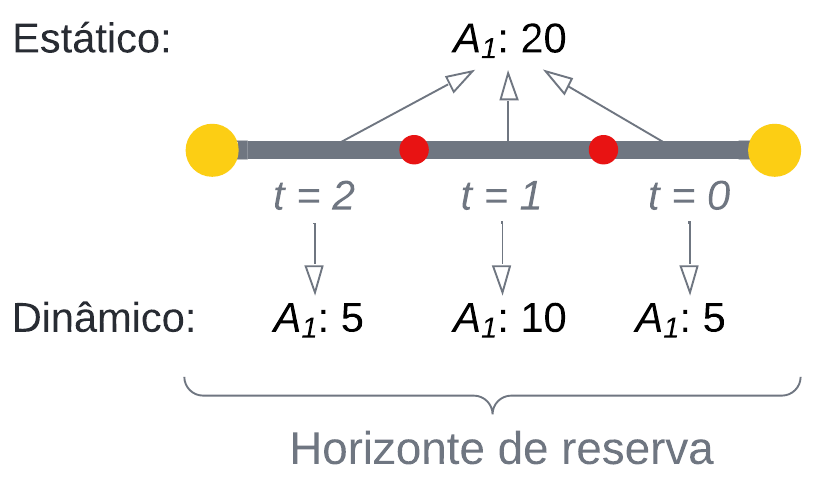
\includegraphics[scale=0.25]{img/classAuto.png}
			\caption{Classes de autorização}
			\label{fig: classAuto}
		\end{center}
	\end{figure}
	\vspace{-1cm}

	\item[Demanda comportamental:] Neste modelo, assume-se que o comportamento de compra dos passageiros é influenciado pelo conjunto de classes de controle disponíveis. Um exemplo desse conceito é ilustrado na Figura \ref{fig: dc1}. Considere um cenário em que 4 clientes desejam comprar a tarifa A3, sendo essa sua primeira opção. Caso a tarifa A3 não esteja disponível, um dos clientes desiste da compra, enquanto os outros 3 permanecem no sistema e estão dispostos a adquirir a tarifa A2. Se A2 também não estiver disponível, mais 2 clientes abandonam a compra, restando apenas um cliente que opta por A1 (geralmente, a opção de maior valor).

	      \begin{figure}[H]
		      \begin{center}
			      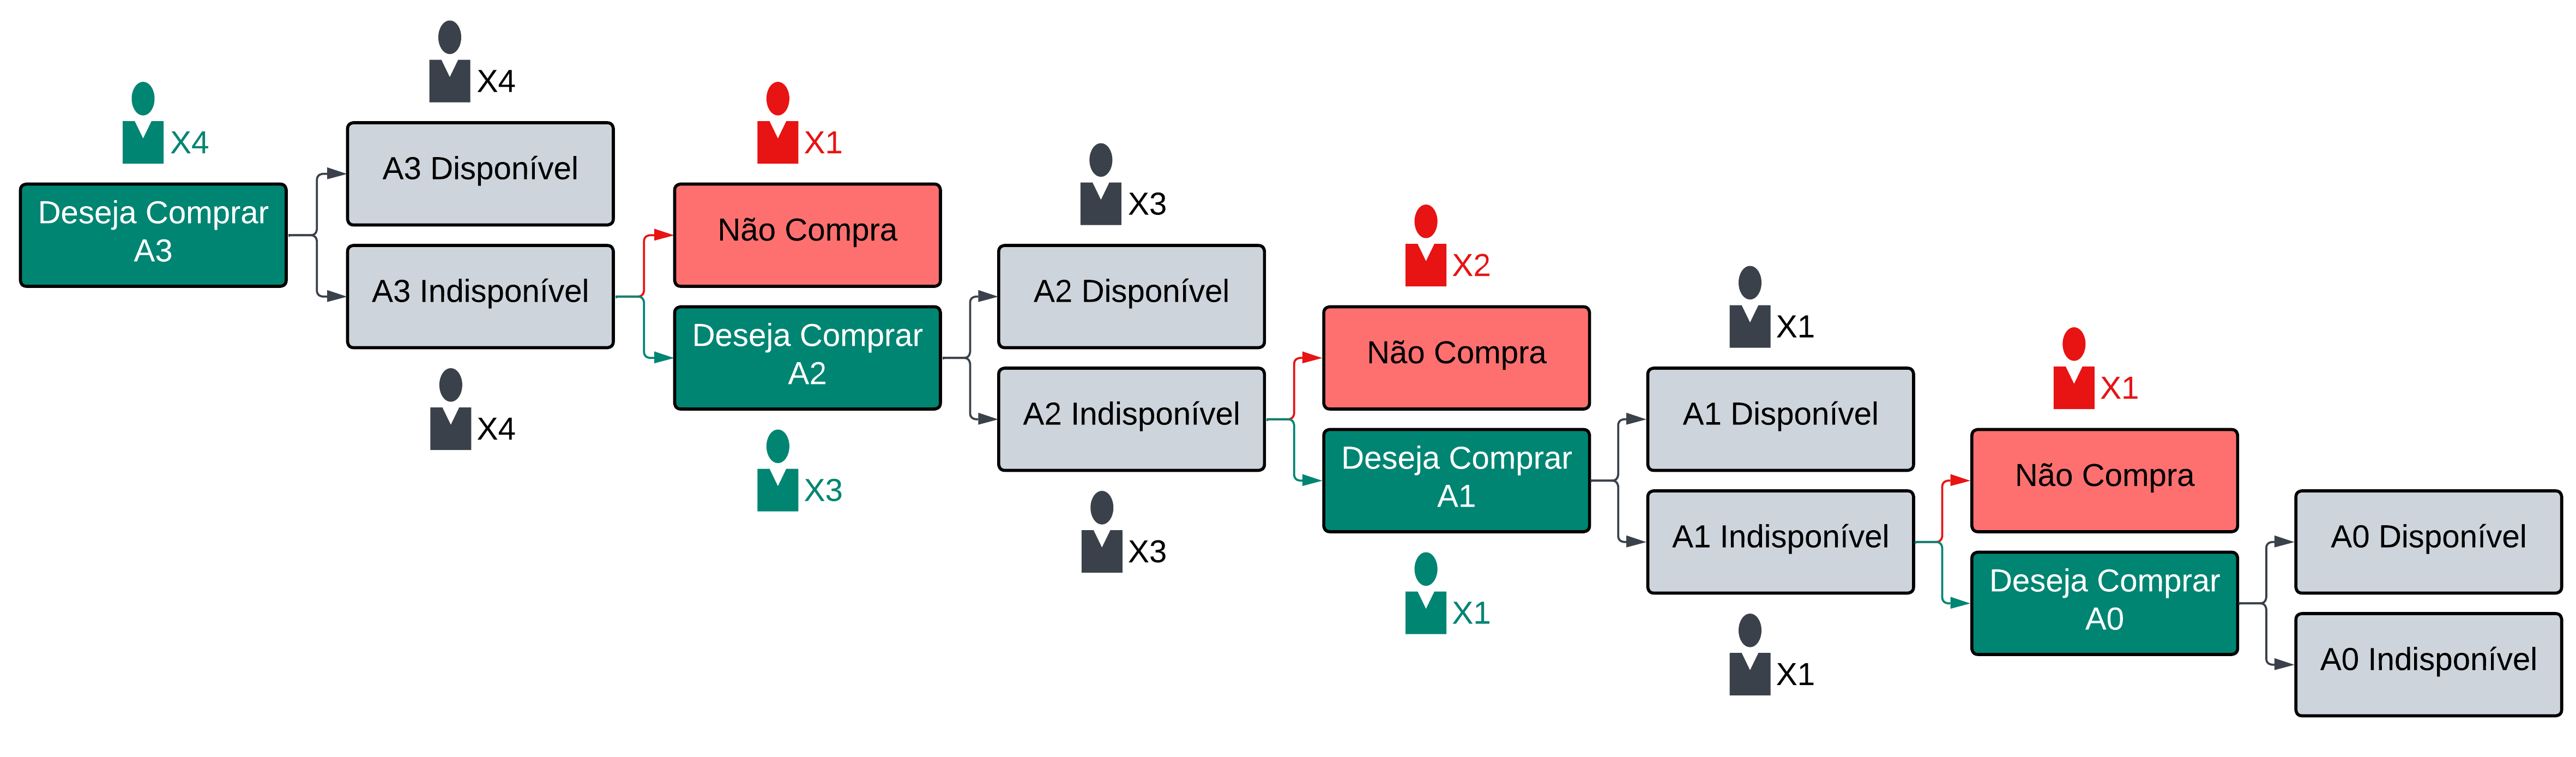
\includegraphics[scale=0.09]{img/dc1.png}
			      \caption{Representação de demanda comportamental}
			      \label{fig: dc1}
		      \end{center}
	      \end{figure}
	      \vspace{-1cm}

	\item[Demanda independente:] Os clientes compram um produto específico, independentemente da oferta disponível no momento. Em um modelo de demanda independente, assume-se que um cliente disposto a pagar R\$100 por um bilhete nunca optaria por um bilhete mais barato (por exemplo, R\$50), mesmo que este estivesse disponível.

	      \begin{figure}[H]
		      \begin{center}
			      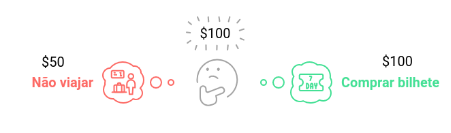
\includegraphics[scale=0.7]{img/di1.png}
			      \caption{Representação de demanda independente}
			      \label{fig: di1}
		      \end{center}
	      \end{figure}
	      \vspace{-1cm}

	\item[Skip lagging:] No contexto do transporte ferroviário de passageiros, skip lagging refere-se a uma estratégia de otimização na programação das paradas dos trens, na qual certos serviços omitem paradas intermediárias em determinados trechos. O objetivo é reduzir os tempos de viagem e aumentar a eficiência operacional, garantindo que essa omissão não comprometa a acessibilidade e a qualidade do serviço oferecido aos passageiros. Na seção de modelagem matemática, será apresentado um conjunto de restrições associadas a esse conceito.

	\item[Fulfillments over periods:] No contexto do transporte ferroviário de passageiros, fulfillments over periods refere-se ao cumprimento de determinados níveis de serviço, demanda ou capacidade ao longo de um período de tempo definido. Esse conceito é especialmente relevante na gestão de receitas, planejamento operacional e alocação de recursos, onde é essencial garantir que a oferta de serviços ferroviários atenda a objetivos estratégicos ao longo do tempo, em vez de se concentrar apenas em momentos específicos. Na seção de modelagem matemática, será apresentado um conjunto de restrições associadas a esse conceito.

	\item[Listas de preferência:] Representam uma hierarquia de alternativas de compra que um passageiro está disposto a considerar no momento da aquisição de uma passagem ferroviária, baseando-se, principalmente, nos preços ofertados nesse momento. Essas listas são fundamentais para entender o comportamento do consumidor e otimizar as estratégias de preços e disponibilidade de assentos. Elas podem ser utilizadas para modelar a demanda de forma mais precisa, levando em conta as preferências dos passageiros e suas reações a diferentes ofertas tarifárias.
\end{description}

\section{Visão geral da pesquisa}

Os problemas relacionados à gestão de receitas (Revenue Management - RM) podem ser definidos como estratégias que visam maximizar as receitas ajustando-se preços e a disponibilidade de capacidade com base na demanda \citep{Gallego1994}. A área de RM foi inicialmente desenvolvida pela indústria aérea nas décadas de 70 e 80, quando as companhias aéreas começaram a adotar técnicas de otimização para definir os preços dos bilhetes com base na disponibilidade de assentos e na antecedência das reservas \citep{article_base}. O objetivo principal do RM consiste em otimizar a disponibilidade e o preço dos produtos para gerar a maior quantidade de receita possível. Entre suas principais características estão a segmentação de clientes, o controle de capacidade, o ajuste dinâmico de preços e o uso de previsões para estimar a demanda. O sucesso alcançado no setor aeronáutico foi tão expressivo que o RM foi expandido para outros setores com características semelhantes, como hotelaria, restaurantes, varejo, comércio eletrônico e transporte \citep{HEO2009446}.

A otimização de receitas no transporte ferroviário de passageiros tornou-se uma área de pesquisa essencial para aumentar a sustentabilidade e a competitividade do setor. Esse tipo de transporte enfrenta desafios específicos na gestão de sua capacidade devido à variabilidade da demanda, à rigidez tarifária e à necessidade crescente de adaptar suas estratégias às dinâmicas de mercado \citep{Guerriero2021}. Nesse contexto, o RM oferece uma estrutura robusta para abordar a alocação ideal de recursos, utilizando técnicas avançadas de modelagem matemática e análise de dados \citep{Ammirato2020}.

O principal objetivo do RM no transporte ferroviário de passageiros pode ser exemplificado da seguinte forma: um operador de transporte define o itinerário de um trem específico, detalhando a origem, o destino e o horário de partida. Os clientes, ou seja, os potenciais passageiros, podem adquirir bilhetes antecipadamente para viajar nesse trem. Chamamos de classes tarifárias ou produtos tarifários os bilhetes disponíveis para venda. O horizonte de reserva é o período de tempo entre a disponibilização inicial dos bilhetes para compra e a partida do trem. Esse horizonte geralmente é dividido em dias, de forma que cada período representa um dia (ou conjunto de dias) antes da partida.

A função do RM, nesse contexto, é controlar a disponibilidade dos produtos tarifários ao longo do horizonte de reserva para maximizar a receita total. Mais especificamente, o processo de otimização busca determinar a quantidade de bilhetes de cada produto que deve estar disponível para venda em cada período, com o objetivo de maximizar os lucros associados a cada partida de trem.

Um elemento fundamental para maximizar as receitas é um modelo preciso da demanda. Alinhar oferta e demanda para otimizar os lucros requer uma compreensão aprofundada do comportamento dos clientes e uma previsão confiável de suas decisões diante de diferentes ofertas de produtos \citep{ZHAO2019776}.

Uma simplificação comum na modelagem da demanda para gestão de receitas é assumir que os clientes têm um comportamento de compra independente. Isso significa que cada cliente compra um produto específico, desconsiderando a oferta disponível no momento. Na prática, por exemplo, um cliente que desejasse comprar um bilhete de trem por R\$10 não pagaria R\$10,50 se essa fosse a única oferta disponível. Em vez disso, ele optaria por não viajar. Da mesma forma, em um modelo de demanda independente, assumimos que um cliente disposto a pagar R\$100 por um bilhete nunca compraria um bilhete mais barato (por exemplo, R\$50), mesmo que estivesse disponível.

Por outro lado, uma abordagem mais robusta considera o comportamento de compra baseado em faixas ou listas de preferência. Esse modelo assume que os clientes escolhem entre um conjunto de ofertas com base em suas preferências. Se a opção mais desejada não estiver disponível, eles passam para a próxima opção viável, desde que esta seja mais atrativa do que não realizar a compra.

Para abordar essa problemática, foram desenvolvidos três modelos de Programação Inteira Mista (MIP): O primeiro baseado em demanda independente. O segundo em demandas comportamentais ajustadas por proporções. Y o terceiro em demandas comportamentais ajustadas por hierarquia.

Esses modelos respeitam as restrições operacionais do sistema ferroviário, como capacidade dos trens, estrutura hierárquica dos produtos tarifários, reservas de bilhetes, disponibilidade de vendas dentro do horizonte de reserva e coerência dos preços dos bilhetes ao longo do tempo, entre outras.

O uso de instâncias reais fornecidas por uma empresa especializada permitiu validar a aplicabilidade dos modelos desenvolvidos, destacando tanto sua capacidade de capturar a complexidade do mercado quanto sua eficiência computacional. Os resultados preliminares indicam que os modelos baseados em demandas comportamentais geraram soluções de melhor qualidade em comparação com o modelo de demanda independente. No entanto, em termos do valor da função objetivo, os modelos comportamentais apresentaram os mesmos resultados entre si, que foram ligeiramente diferentes dos obtidos pelo modelo independente.

Essa pesquisa contribui para o corpo de conhecimento em Revenue Management ao combinar técnicas de modelagem baseadas em demandas comportamentais, utilizando listas de preferência, e programação matemática para resolver problemas complexos de alocação de assentos no transporte ferroviário de passageiros.
% \end{quotation}